% This is part of Exercices et corrigés de CdI-1
% Copyright (c) 2011-2012,2016
%   Laurent Claessens
% See the file fdl-1.3.txt for copying conditions.

\begin{exercice}\label{exoTP20090003}


Considérons un tore $T$ dans $\eR^3$, c’est-à-dire la surface de révolution engendrée par la rotation d’un cercle de rayon $r$ autour d’un axe coplanaire et disjoint de ce cercle, à distance $R$ du centre du cercle.
\begin{enumerate}

	\item
		Donner une paramétrisation du tore en fonction de deux angles $\varphi$ et $\theta$ bien choisis (la figure \ref{FigToreWiki} devrait vous aider).
	\item
		Donner une carte autour d’un point $(x_0 , y_0 , z_0 )$ sur le tore et vérifier les conditions de la définition de variété sous forme paramétrique.
	\item
		Écrire l'équation du plan tangent au tore au point $(x_0 , y_0 , z_0 )$.
	\item
		Calculer le volume intérieur au tore.

\end{enumerate}

\begin{figure}
	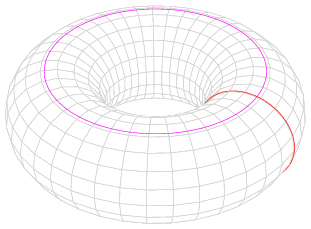
\includegraphics[width=5cm]{pictures_bitmap/Torus_cycles.png}
	\caption{Les cercles du tore, figure de \href{http://fr.wikipedia.org/wiki/Tore}{wikipedia}.}\label{FigToreWiki}
\end{figure}

\corrref{TP20090003}
\end{exercice}
